\documentclass[1p]{elsarticle_modified}
%\bibliographystyle{elsarticle-num}

%\usepackage[colorlinks]{hyperref}
%\usepackage{abbrmath_seonhwa} %\Abb, \Ascr, \Acal ,\Abf, \Afrak
\usepackage{amsfonts}
\usepackage{amssymb}
\usepackage{amsmath}
\usepackage{amsthm}
\usepackage{scalefnt}
\usepackage{amsbsy}
\usepackage{kotex}
\usepackage{caption}
\usepackage{subfig}
\usepackage{color}
\usepackage{graphicx}
\usepackage{xcolor} %% white, black, red, green, blue, cyan, magenta, yellow
\usepackage{float}
\usepackage{setspace}
\usepackage{hyperref}

\usepackage{tikz}
\usetikzlibrary{arrows}

\usepackage{multirow}
\usepackage{array} % fixed length table
\usepackage{hhline}

%%%%%%%%%%%%%%%%%%%%%
\makeatletter
\renewcommand*\env@matrix[1][\arraystretch]{%
	\edef\arraystretch{#1}%
	\hskip -\arraycolsep
	\let\@ifnextchar\new@ifnextchar
	\array{*\c@MaxMatrixCols c}}
\makeatother %https://tex.stackexchange.com/questions/14071/how-can-i-increase-the-line-spacing-in-a-matrix
%%%%%%%%%%%%%%%

\usepackage[normalem]{ulem}

\newcommand{\msout}[1]{\ifmmode\text{\sout{\ensuremath{#1}}}\else\sout{#1}\fi}
%SOURCE: \msout is \stkout macro in https://tex.stackexchange.com/questions/20609/strikeout-in-math-mode

\newcommand{\cancel}[1]{
	\ifmmode
	{\color{red}\msout{#1}}
	\else
	{\color{red}\sout{#1}}
	\fi
}

\newcommand{\add}[1]{
	{\color{blue}\uwave{#1}}
}

\newcommand{\replace}[2]{
	\ifmmode
	{\color{red}\msout{#1}}{\color{blue}\uwave{#2}}
	\else
	{\color{red}\sout{#1}}{\color{blue}\uwave{#2}}
	\fi
}

\newcommand{\Sol}{\mathcal{S}} %segment
\newcommand{\D}{D} %diagram
\newcommand{\A}{\mathcal{A}} %arc


%%%%%%%%%%%%%%%%%%%%%%%%%%%%%5 test

\def\sl{\operatorname{\textup{SL}}(2,\Cbb)}
\def\psl{\operatorname{\textup{PSL}}(2,\Cbb)}
\def\quan{\mkern 1mu \triangleright \mkern 1mu}

\theoremstyle{definition}
\newtheorem{thm}{Theorem}[section]
\newtheorem{prop}[thm]{Proposition}
\newtheorem{lem}[thm]{Lemma}
\newtheorem{ques}[thm]{Question}
\newtheorem{cor}[thm]{Corollary}
\newtheorem{defn}[thm]{Definition}
\newtheorem{exam}[thm]{Example}
\newtheorem{rmk}[thm]{Remark}
\newtheorem{alg}[thm]{Algorithm}

\newcommand{\I}{\sqrt{-1}}
\begin{document}

%\begin{frontmatter}
%
%\title{Boundary parabolic representations of knots up to 8 crossings}
%
%%% Group authors per affiliation:
%\author{Yunhi Cho} 
%\address{Department of Mathematics, University of Seoul, Seoul, Korea}
%\ead{yhcho@uos.ac.kr}
%
%
%\author{Seonhwa Kim} %\fnref{s_kim}}
%\address{Center for Geometry and Physics, Institute for Basic Science, Pohang, 37673, Korea}
%\ead{ryeona17@ibs.re.kr}
%
%\author{Hyuk Kim}
%\address{Department of Mathematical Sciences, Seoul National University, Seoul 08826, Korea}
%\ead{hyukkim@snu.ac.kr}
%
%\author{Seokbeom Yoon}
%\address{Department of Mathematical Sciences, Seoul National University, Seoul, 08826,  Korea}
%\ead{sbyoon15@snu.ac.kr}
%
%\begin{abstract}
%We find all boundary parabolic representation of knots up to 8 crossings.
%
%\end{abstract}
%\begin{keyword}
%    \MSC[2010] 57M25 
%\end{keyword}
%
%\end{frontmatter}

%\linenumbers
%\tableofcontents
%
\newcommand\colored[1]{\textcolor{white}{\rule[-0.35ex]{0.8em}{1.4ex}}\kern-0.8em\color{red} #1}%
%\newcommand\colored[1]{\textcolor{white}{ #1}\kern-2.17ex	\textcolor{white}{ #1}\kern-1.81ex	\textcolor{white}{ #1}\kern-2.15ex\color{red}#1	}

{\Large $\underline{12a_{0286}~(K12a_{0286})}$}

\setlength{\tabcolsep}{10pt}
\renewcommand{\arraystretch}{1.6}
\vspace{1cm}\begin{tabular}{m{100pt}>{\centering\arraybackslash}m{274pt}}
\multirow{5}{120pt}{
	\centering
	\includegraphics[width=112pt]{../../../GIT/diagram.site/Diagrams/png/1087_12a_0286.png}\\
\ \ \ A knot diagram\footnotemark}&
\allowdisplaybreaks
\textbf{Linearized knot diagam} \\
\cline{2-2}
 &
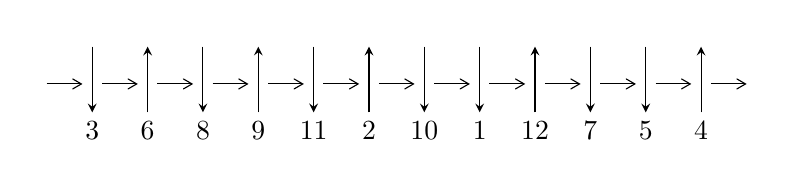
\begin{tikzpicture}[x=20pt, y=17pt]
	% nodes
	\node (C0) at (0, 0) {};
	\node (C1) at (1, 0) {};
	\node (C1U) at (1, +1) {};
	\node (C1D) at (1, -1) {3};

	\node (C2) at (2, 0) {};
	\node (C2U) at (2, +1) {};
	\node (C2D) at (2, -1) {6};

	\node (C3) at (3, 0) {};
	\node (C3U) at (3, +1) {};
	\node (C3D) at (3, -1) {8};

	\node (C4) at (4, 0) {};
	\node (C4U) at (4, +1) {};
	\node (C4D) at (4, -1) {9};

	\node (C5) at (5, 0) {};
	\node (C5U) at (5, +1) {};
	\node (C5D) at (5, -1) {11};

	\node (C6) at (6, 0) {};
	\node (C6U) at (6, +1) {};
	\node (C6D) at (6, -1) {2};

	\node (C7) at (7, 0) {};
	\node (C7U) at (7, +1) {};
	\node (C7D) at (7, -1) {10};

	\node (C8) at (8, 0) {};
	\node (C8U) at (8, +1) {};
	\node (C8D) at (8, -1) {1};

	\node (C9) at (9, 0) {};
	\node (C9U) at (9, +1) {};
	\node (C9D) at (9, -1) {12};

	\node (C10) at (10, 0) {};
	\node (C10U) at (10, +1) {};
	\node (C10D) at (10, -1) {7};

	\node (C11) at (11, 0) {};
	\node (C11U) at (11, +1) {};
	\node (C11D) at (11, -1) {5};

	\node (C12) at (12, 0) {};
	\node (C12U) at (12, +1) {};
	\node (C12D) at (12, -1) {4};
	\node (C13) at (13, 0) {};

	% arrows
	\draw[->,>={angle 60}]
	(C0) edge (C1) (C1) edge (C2) (C2) edge (C3) (C3) edge (C4) (C4) edge (C5) (C5) edge (C6) (C6) edge (C7) (C7) edge (C8) (C8) edge (C9) (C9) edge (C10) (C10) edge (C11) (C11) edge (C12) (C12) edge (C13) ;	\draw[->,>=stealth]
	(C1U) edge (C1D) (C2D) edge (C2U) (C3U) edge (C3D) (C4D) edge (C4U) (C5U) edge (C5D) (C6D) edge (C6U) (C7U) edge (C7D) (C8U) edge (C8D) (C9D) edge (C9U) (C10U) edge (C10D) (C11U) edge (C11D) (C12D) edge (C12U) ;
	\end{tikzpicture} \\
\hhline{~~} \\& 
\textbf{Solving Sequence} \\ \cline{2-2} 
 &
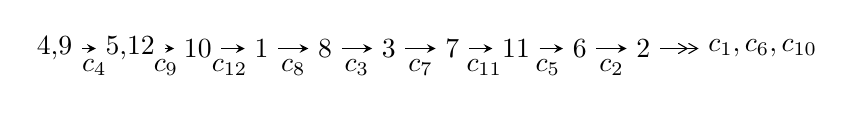
\begin{tikzpicture}[x=23pt, y=7pt]
	% node
	\node (A0) at (-1/8, 0) {4,9};
	\node (A1) at (17/16, 0) {5,12};
	\node (A2) at (17/8, 0) {10};
	\node (A3) at (25/8, 0) {1};
	\node (A4) at (33/8, 0) {8};
	\node (A5) at (41/8, 0) {3};
	\node (A6) at (49/8, 0) {7};
	\node (A7) at (57/8, 0) {11};
	\node (A8) at (65/8, 0) {6};
	\node (A9) at (73/8, 0) {2};
	\node (C1) at (1/2, -1) {$c_{4}$};
	\node (C2) at (13/8, -1) {$c_{9}$};
	\node (C3) at (21/8, -1) {$c_{12}$};
	\node (C4) at (29/8, -1) {$c_{8}$};
	\node (C5) at (37/8, -1) {$c_{3}$};
	\node (C6) at (45/8, -1) {$c_{7}$};
	\node (C7) at (53/8, -1) {$c_{11}$};
	\node (C8) at (61/8, -1) {$c_{5}$};
	\node (C9) at (69/8, -1) {$c_{2}$};
	\node (A10) at (11, 0) {$c_{1},c_{6},c_{10}$};

	% edge
	\draw[->,>=stealth]	
	(A0) edge (A1) (A1) edge (A2) (A2) edge (A3) (A3) edge (A4) (A4) edge (A5) (A5) edge (A6) (A6) edge (A7) (A7) edge (A8) (A8) edge (A9) ;
	\draw[->>,>={angle 60}]	
	(A9) edge (A10);
\end{tikzpicture} \\ 

\end{tabular} \\

\footnotetext{
The image of knot diagram is generated by the software ``\textbf{Draw programme}" developed by Andrew Bartholomew(\url{http://www.layer8.co.uk/maths/draw/index.htm\#Running-draw}), where we modified some parts for our purpose(\url{https://github.com/CATsTAILs/LinksPainter}).
}\phantom \\ \newline 
\centering \textbf{Ideals for irreducible components\footnotemark of $X_{\text{par}}$} 
 
\begin{align*}
I^u_{1}&=\langle 
-1.08457\times10^{28} u^{31}-9.68465\times10^{27} u^{30}+\cdots+3.30621\times10^{28} b+6.26853\times10^{28},\\
\phantom{I^u_{1}}&\phantom{= \langle  }1.00919\times10^{29} u^{31}-4.41562\times10^{28} u^{30}+\cdots+3.30621\times10^{28} a+4.42115\times10^{28},\;u^{32}-2 u^{30}+\cdots+2 u+1\rangle \\
I^u_{2}&=\langle 
- u^3+u^2+4 b-5 u+2,\;a,\;u^4- u^3+5 u^2-2 u+4\rangle \\
\\
\end{align*}
\raggedright * 2 irreducible components of $\dim_{\mathbb{C}}=0$, with total 36 representations.\\
\footnotetext{All coefficients of polynomials are rational numbers. But the coefficients are sometimes approximated in decimal forms when there is not enough margin.}
\newpage
\renewcommand{\arraystretch}{1}
\centering \section*{I. $I^u_{1}= \langle -1.08\times10^{28} u^{31}-9.68\times10^{27} u^{30}+\cdots+3.31\times10^{28} b+6.27\times10^{28},\;1.01\times10^{29} u^{31}-4.42\times10^{28} u^{30}+\cdots+3.31\times10^{28} a+4.42\times10^{28},\;u^{32}-2 u^{30}+\cdots+2 u+1 \rangle$}
\flushleft \textbf{(i) Arc colorings}\\
\begin{tabular}{m{7pt} m{180pt} m{7pt} m{180pt} }
\flushright $a_{4}=$&$\begin{pmatrix}1\\0\end{pmatrix}$ \\
\flushright $a_{9}=$&$\begin{pmatrix}0\\u\end{pmatrix}$ \\
\flushright $a_{5}=$&$\begin{pmatrix}1\\- u^2\end{pmatrix}$ \\
\flushright $a_{12}=$&$\begin{pmatrix}-3.05243 u^{31}+1.33556 u^{30}+\cdots-5.33264 u-1.33723\\0.328041 u^{31}+0.292923 u^{30}+\cdots+0.733300 u-1.89599\end{pmatrix}$ \\
\flushright $a_{10}=$&$\begin{pmatrix}6.38763 u^{31}-3.08529 u^{30}+\cdots+7.92825 u+8.64307\\-0.227028 u^{31}+0.570345 u^{30}+\cdots-1.64514 u+1.43963\end{pmatrix}$ \\
\flushright $a_{1}=$&$\begin{pmatrix}-2.72438 u^{31}+1.62848 u^{30}+\cdots-4.59934 u-3.23322\\0.328041 u^{31}+0.292923 u^{30}+\cdots+0.733300 u-1.89599\end{pmatrix}$ \\
\flushright $a_{8}=$&$\begin{pmatrix}5.67422 u^{31}-2.13572 u^{30}+\cdots+1.41383 u+9.56776\\-0.486384 u^{31}+0.379216 u^{30}+\cdots-2.86928 u-0.514941\end{pmatrix}$ \\
\flushright $a_{3}=$&$\begin{pmatrix}-3.24515 u^{31}+1.67422 u^{30}+\cdots-3.02690 u-4.97838\\0.304612 u^{31}-0.193228 u^{30}+\cdots+3.65994 u-0.679133\end{pmatrix}$ \\
\flushright $a_{7}=$&$\begin{pmatrix}7.00844 u^{31}-0.808937 u^{30}+\cdots-7.09680 u+17.1331\\-2.34735 u^{31}-0.0978616 u^{30}+\cdots-1.67702 u-2.05955\end{pmatrix}$ \\
\flushright $a_{11}=$&$\begin{pmatrix}-3.95240 u^{31}+1.64688 u^{30}+\cdots-4.21803 u-4.56877\\0.349246 u^{31}+0.484634 u^{30}+\cdots+0.455964 u-1.58467\end{pmatrix}$ \\
\flushright $a_{6}=$&$\begin{pmatrix}-2.33177 u^{31}+0.938856 u^{30}+\cdots+3.06552 u-9.72970\\2.18533 u^{31}-0.590773 u^{30}+\cdots+3.26730 u+2.12120\end{pmatrix}$ \\
\flushright $a_{2}=$&$\begin{pmatrix}-8.37149 u^{31}+5.01296 u^{30}+\cdots-12.6435 u-10.7929\\-1.24677 u^{31}-0.611740 u^{30}+\cdots+8.72740 u-2.92118\end{pmatrix}$\\&\end{tabular}
\flushleft \textbf{(ii) Obstruction class $= 1$}\\~\\
\flushleft \textbf{(iii) Cusp Shapes $= 4.80290 u^{31}-0.110659 u^{30}+\cdots-8.67744 u+4.28329$}\\~\\
\newpage\renewcommand{\arraystretch}{1}
\flushleft \textbf{(iv) u-Polynomials at the component}\newline \\
\begin{tabular}{m{50pt}|m{274pt}}
Crossings & \hspace{64pt}u-Polynomials at each crossing \\
\hline $$\begin{aligned}c_{1}\end{aligned}$$&$\begin{aligned}
&u^{32}-16 u^{31}+\cdots-10 u+1
\end{aligned}$\\
\hline $$\begin{aligned}c_{2}\end{aligned}$$&$\begin{aligned}
&u^{32}-4 u^{31}+\cdots-6 u+1
\end{aligned}$\\
\hline $$\begin{aligned}c_{3}\end{aligned}$$&$\begin{aligned}
&u^{32}+8 u^{30}+\cdots+6 u+1
\end{aligned}$\\
\hline $$\begin{aligned}c_{4}\end{aligned}$$&$\begin{aligned}
&u^{32}-2 u^{30}+\cdots+2 u+1
\end{aligned}$\\
\hline $$\begin{aligned}c_{5}\end{aligned}$$&$\begin{aligned}
&u^{32}-4 u^{31}+\cdots+8 u+1
\end{aligned}$\\
\hline $$\begin{aligned}c_{6}\end{aligned}$$&$\begin{aligned}
&u^{32}+4 u^{31}+\cdots+6 u+1
\end{aligned}$\\
\hline $$\begin{aligned}c_{7}\end{aligned}$$&$\begin{aligned}
&u^{32}-10 u^{31}+\cdots-2 u+1
\end{aligned}$\\
\hline $$\begin{aligned}c_{8}\end{aligned}$$&$\begin{aligned}
&u^{32}+6 u^{31}+\cdots+4 u+1
\end{aligned}$\\
\hline $$\begin{aligned}c_{9}\end{aligned}$$&$\begin{aligned}
&u^{32}+10 u^{31}+\cdots+538 u+73
\end{aligned}$\\
\hline $$\begin{aligned}c_{10}\end{aligned}$$&$\begin{aligned}
&u^{32}+10 u^{31}+\cdots+2 u+1
\end{aligned}$\\
\hline $$\begin{aligned}c_{11}\end{aligned}$$&$\begin{aligned}
&u^{32}+4 u^{31}+\cdots-8 u+1
\end{aligned}$\\
\hline $$\begin{aligned}c_{12}\end{aligned}$$&$\begin{aligned}
&u^{32}+4 u^{31}+\cdots-2 u+1
\end{aligned}$\\
\hline
\end{tabular}\\~\\
\newpage\renewcommand{\arraystretch}{1}
\flushleft \textbf{(v) Riley Polynomials at the component}\newline \\
\begin{tabular}{m{50pt}|m{274pt}}
Crossings & \hspace{64pt}Riley Polynomials at each crossing \\
\hline $$\begin{aligned}c_{1}\end{aligned}$$&$\begin{aligned}
&y^{32}+4 y^{31}+\cdots+10 y+1
\end{aligned}$\\
\hline $$\begin{aligned}c_{2},c_{6}\end{aligned}$$&$\begin{aligned}
&y^{32}+16 y^{31}+\cdots+10 y+1
\end{aligned}$\\
\hline $$\begin{aligned}c_{3}\end{aligned}$$&$\begin{aligned}
&y^{32}+16 y^{31}+\cdots-12 y+1
\end{aligned}$\\
\hline $$\begin{aligned}c_{4}\end{aligned}$$&$\begin{aligned}
&y^{32}-4 y^{31}+\cdots-16 y+1
\end{aligned}$\\
\hline $$\begin{aligned}c_{5},c_{11}\end{aligned}$$&$\begin{aligned}
&y^{32}+20 y^{31}+\cdots+16 y+1
\end{aligned}$\\
\hline $$\begin{aligned}c_{7},c_{10}\end{aligned}$$&$\begin{aligned}
&y^{32}+18 y^{31}+\cdots+22 y+1
\end{aligned}$\\
\hline $$\begin{aligned}c_{8}\end{aligned}$$&$\begin{aligned}
&y^{32}-12 y^{31}+\cdots+14 y+1
\end{aligned}$\\
\hline $$\begin{aligned}c_{9}\end{aligned}$$&$\begin{aligned}
&y^{32}-14 y^{31}+\cdots+77162 y+5329
\end{aligned}$\\
\hline $$\begin{aligned}c_{12}\end{aligned}$$&$\begin{aligned}
&y^{32}-4 y^{31}+\cdots+20 y+1
\end{aligned}$\\
\hline
\end{tabular}\\~\\
\newpage\flushleft \textbf{(vi) Complex Volumes and Cusp Shapes}
$$\begin{array}{c|c|c}  
\text{Solutions to }I^u_{1}& \I (\text{vol} + \sqrt{-1}CS) & \text{Cusp shape}\\
 \hline 
\begin{aligned}
u &= -1.011430 + 0.076540 I \\
a &= -0.299553 - 1.057440 I \\
b &= \phantom{-}0.066450 + 1.277390 I\end{aligned}
 & \phantom{-}1.95636 + 4.51992 I & -2.62248 - 7.58475 I \\ \hline\begin{aligned}
u &= -1.011430 - 0.076540 I \\
a &= -0.299553 + 1.057440 I \\
b &= \phantom{-}0.066450 - 1.277390 I\end{aligned}
 & \phantom{-}1.95636 - 4.51992 I & -2.62248 + 7.58475 I \\ \hline\begin{aligned}
u &= -0.195501 + 0.960625 I \\
a &= -0.54851 - 1.43505 I \\
b &= -0.037707 - 0.482351 I\end{aligned}
 & -1.46529 - 0.97885 I & -11.84592 - 4.46110 I \\ \hline\begin{aligned}
u &= -0.195501 - 0.960625 I \\
a &= -0.54851 + 1.43505 I \\
b &= -0.037707 + 0.482351 I\end{aligned}
 & -1.46529 + 0.97885 I & -11.84592 + 4.46110 I \\ \hline\begin{aligned}
u &= \phantom{-}0.963349 + 0.082588 I \\
a &= \phantom{-}0.874463 + 0.489100 I \\
b &= -1.056860 - 0.880917 I\end{aligned}
 & \phantom{-}0.52518 - 1.70904 I & \phantom{-}1.303152 + 0.227505 I \\ \hline\begin{aligned}
u &= \phantom{-}0.963349 - 0.082588 I \\
a &= \phantom{-}0.874463 - 0.489100 I \\
b &= -1.056860 + 0.880917 I\end{aligned}
 & \phantom{-}0.52518 + 1.70904 I & \phantom{-}1.303152 - 0.227505 I \\ \hline\begin{aligned}
u &= \phantom{-}0.897933 + 0.134537 I \\
a &= -0.079600 - 1.057370 I \\
b &= -0.417549 + 0.423958 I\end{aligned}
 & -1.93841 - 3.89093 I & -2.89352 + 9.56275 I \\ \hline\begin{aligned}
u &= \phantom{-}0.897933 - 0.134537 I \\
a &= -0.079600 + 1.057370 I \\
b &= -0.417549 - 0.423958 I\end{aligned}
 & -1.93841 + 3.89093 I & -2.89352 - 9.56275 I \\ \hline\begin{aligned}
u &= -0.790801 + 0.178174 I \\
a &= -1.07264 + 1.31010 I \\
b &= \phantom{-}0.144360 - 0.486258 I\end{aligned}
 & -1.66071 - 1.88565 I & \phantom{-}0.611617 + 0.405112 I \\ \hline\begin{aligned}
u &= -0.790801 - 0.178174 I \\
a &= -1.07264 - 1.31010 I \\
b &= \phantom{-}0.144360 + 0.486258 I\end{aligned}
 & -1.66071 + 1.88565 I & \phantom{-}0.611617 - 0.405112 I\\
 \hline 
 \end{array}$$\newpage$$\begin{array}{c|c|c}  
\text{Solutions to }I^u_{1}& \I (\text{vol} + \sqrt{-1}CS) & \text{Cusp shape}\\
 \hline 
\begin{aligned}
u &= \phantom{-}0.725473 + 0.306578 I \\
a &= \phantom{-}2.59490 + 0.04955 I \\
b &= -1.370940 - 0.282852 I\end{aligned}
 & -0.233393 + 0.291097 I & -5.20473 + 2.81677 I \\ \hline\begin{aligned}
u &= \phantom{-}0.725473 - 0.306578 I \\
a &= \phantom{-}2.59490 - 0.04955 I \\
b &= -1.370940 + 0.282852 I\end{aligned}
 & -0.233393 - 0.291097 I & -5.20473 - 2.81677 I \\ \hline\begin{aligned}
u &= -0.358787 + 1.159020 I \\
a &= \phantom{-}0.506557 + 0.930883 I \\
b &= -0.576105 + 0.212433 I\end{aligned}
 & \phantom{-}7.03446 - 10.43960 I & \phantom{-}3.24799 + 7.92017 I \\ \hline\begin{aligned}
u &= -0.358787 - 1.159020 I \\
a &= \phantom{-}0.506557 - 0.930883 I \\
b &= -0.576105 - 0.212433 I\end{aligned}
 & \phantom{-}7.03446 + 10.43960 I & \phantom{-}3.24799 - 7.92017 I \\ \hline\begin{aligned}
u &= -1.236250 + 0.423599 I \\
a &= -1.23017 + 0.89428 I \\
b &= \phantom{-}1.08185 - 1.47183 I\end{aligned}
 & \phantom{-}4.04750 - 6.51115 I & \phantom{-}7.4827 + 17.7604 I \\ \hline\begin{aligned}
u &= -1.236250 - 0.423599 I \\
a &= -1.23017 - 0.89428 I \\
b &= \phantom{-}1.08185 + 1.47183 I\end{aligned}
 & \phantom{-}4.04750 + 6.51115 I & \phantom{-}7.4827 - 17.7604 I \\ \hline\begin{aligned}
u &= \phantom{-}0.754987 + 1.099260 I \\
a &= -0.851878 + 0.547278 I \\
b &= \phantom{-}0.676413 + 0.328413 I\end{aligned}
 & \phantom{-}8.54048 + 4.66147 I & \phantom{-}5.60896 - 3.18468 I \\ \hline\begin{aligned}
u &= \phantom{-}0.754987 - 1.099260 I \\
a &= -0.851878 - 0.547278 I \\
b &= \phantom{-}0.676413 - 0.328413 I\end{aligned}
 & \phantom{-}8.54048 - 4.66147 I & \phantom{-}5.60896 + 3.18468 I \\ \hline\begin{aligned}
u &= -0.541157 + 0.373122 I \\
a &= -0.611032 - 0.446290 I \\
b &= \phantom{-}1.48390 - 0.85410 I\end{aligned}
 & \phantom{-}2.56066 - 1.39415 I & \phantom{-}8.59786 - 1.04596 I \\ \hline\begin{aligned}
u &= -0.541157 - 0.373122 I \\
a &= -0.611032 + 0.446290 I \\
b &= \phantom{-}1.48390 + 0.85410 I\end{aligned}
 & \phantom{-}2.56066 + 1.39415 I & \phantom{-}8.59786 + 1.04596 I\\
 \hline 
 \end{array}$$\newpage$$\begin{array}{c|c|c}  
\text{Solutions to }I^u_{1}& \I (\text{vol} + \sqrt{-1}CS) & \text{Cusp shape}\\
 \hline 
\begin{aligned}
u &= \phantom{-}1.078990 + 0.816307 I \\
a &= \phantom{-}1.071980 - 0.021161 I \\
b &= -1.00062 - 1.06785 I\end{aligned}
 & \phantom{-}0.04554 + 9.55039 I & \phantom{-}0.17757 - 7.82747 I \\ \hline\begin{aligned}
u &= \phantom{-}1.078990 - 0.816307 I \\
a &= \phantom{-}1.071980 + 0.021161 I \\
b &= -1.00062 + 1.06785 I\end{aligned}
 & \phantom{-}0.04554 - 9.55039 I & \phantom{-}0.17757 + 7.82747 I \\ \hline\begin{aligned}
u &= \phantom{-}0.349670 + 0.386213 I \\
a &= -0.448966 - 0.257825 I \\
b &= \phantom{-}1.82694 + 1.31311 I\end{aligned}
 & \phantom{-}3.77595 + 1.55640 I & -10.9090 - 16.7964 I \\ \hline\begin{aligned}
u &= \phantom{-}0.349670 - 0.386213 I \\
a &= -0.448966 + 0.257825 I \\
b &= \phantom{-}1.82694 - 1.31311 I\end{aligned}
 & \phantom{-}3.77595 - 1.55640 I & -10.9090 + 16.7964 I \\ \hline\begin{aligned}
u &= \phantom{-}1.21893 + 0.86163 I \\
a &= -0.997262 - 0.051859 I \\
b &= \phantom{-}0.766581 + 0.643238 I\end{aligned}
 & \phantom{-}7.91161 + 4.63893 I & \phantom{-}7.21423 - 8.93330 I \\ \hline\begin{aligned}
u &= \phantom{-}1.21893 - 0.86163 I \\
a &= -0.997262 + 0.051859 I \\
b &= \phantom{-}0.766581 - 0.643238 I\end{aligned}
 & \phantom{-}7.91161 - 4.63893 I & \phantom{-}7.21423 + 8.93330 I \\ \hline\begin{aligned}
u &= -1.27730 + 0.81643 I \\
a &= -0.841795 + 0.203609 I \\
b &= \phantom{-}0.93799 - 1.07457 I\end{aligned}
 & \phantom{-}2.06970 - 6.21261 I & -3.30852 + 0. I\phantom{ +0.000000I} \\ \hline\begin{aligned}
u &= -1.27730 - 0.81643 I \\
a &= -0.841795 - 0.203609 I \\
b &= \phantom{-}0.93799 + 1.07457 I\end{aligned}
 & \phantom{-}2.06970 + 6.21261 I & -3.30852 + 0. I\phantom{ +0.000000I} \\ \hline\begin{aligned}
u &= -0.435914 + 0.191346 I \\
a &= \phantom{-}3.01618 - 0.43588 I \\
b &= -0.516431 - 0.791322 I\end{aligned}
 & \phantom{-}1.57422 - 2.11475 I & \phantom{-}0.389556 + 1.338497 I \\ \hline\begin{aligned}
u &= -0.435914 - 0.191346 I \\
a &= \phantom{-}3.01618 + 0.43588 I \\
b &= -0.516431 + 0.791322 I\end{aligned}
 & \phantom{-}1.57422 + 2.11475 I & \phantom{-}0.389556 - 1.338497 I\\
 \hline 
 \end{array}$$\newpage$$\begin{array}{c|c|c}  
\text{Solutions to }I^u_{1}& \I (\text{vol} + \sqrt{-1}CS) & \text{Cusp shape}\\
 \hline 
\begin{aligned}
u &= -0.14221 + 1.69421 I \\
a &= -0.082679 - 0.594170 I \\
b &= -0.008276 - 0.433413 I\end{aligned}
 & \phantom{-}1.44470 + 2.66235 I & \phantom{-}7.15055 - 3.68105 I \\ \hline\begin{aligned}
u &= -0.14221 - 1.69421 I \\
a &= -0.082679 + 0.594170 I \\
b &= -0.008276 + 0.433413 I\end{aligned}
 & \phantom{-}1.44470 - 2.66235 I & \phantom{-}7.15055 + 3.68105 I\\
 \hline 
 \end{array}$$\newpage\newpage\renewcommand{\arraystretch}{1}
\centering \section*{II. $I^u_{2}= \langle - u^3+u^2+4 b-5 u+2,\;a,\;u^4- u^3+5 u^2-2 u+4 \rangle$}
\flushleft \textbf{(i) Arc colorings}\\
\begin{tabular}{m{7pt} m{180pt} m{7pt} m{180pt} }
\flushright $a_{4}=$&$\begin{pmatrix}1\\0\end{pmatrix}$ \\
\flushright $a_{9}=$&$\begin{pmatrix}0\\u\end{pmatrix}$ \\
\flushright $a_{5}=$&$\begin{pmatrix}1\\- u^2\end{pmatrix}$ \\
\flushright $a_{12}=$&$\begin{pmatrix}0\\\frac{1}{4} u^3-\frac{1}{4} u^2+\frac{5}{4} u-\frac{1}{2}\end{pmatrix}$ \\
\flushright $a_{10}=$&$\begin{pmatrix}0\\u\end{pmatrix}$ \\
\flushright $a_{1}=$&$\begin{pmatrix}\frac{1}{4} u^3-\frac{1}{4} u^2+\frac{5}{4} u-\frac{1}{2}\\\frac{1}{4} u^3-\frac{1}{4} u^2+\frac{5}{4} u-\frac{1}{2}\end{pmatrix}$ \\
\flushright $a_{8}=$&$\begin{pmatrix}-\frac{1}{4} u^3+\frac{1}{4} u^2-\frac{5}{4} u+\frac{1}{2}\\-\frac{1}{4} u^3+\frac{1}{4} u^2-\frac{1}{4} u+\frac{1}{2}\end{pmatrix}$ \\
\flushright $a_{3}=$&$\begin{pmatrix}\frac{1}{8} u^3+\frac{1}{8} u^2+\frac{3}{8} u+1\\\frac{1}{8} u^3-\frac{7}{8} u^2+\frac{3}{8} u-1\end{pmatrix}$ \\
\flushright $a_{7}=$&$\begin{pmatrix}-\frac{1}{4} u^3+\frac{1}{4} u^2-\frac{5}{4} u+\frac{1}{2}\\-\frac{1}{4} u^3+\frac{1}{4} u^2-\frac{5}{4} u+\frac{1}{2}\end{pmatrix}$ \\
\flushright $a_{11}=$&$\begin{pmatrix}\frac{1}{4} u^3-\frac{1}{4} u^2+\frac{5}{4} u-\frac{1}{2}\\\frac{1}{4} u^3-\frac{1}{4} u^2+\frac{9}{4} u-\frac{1}{2}\end{pmatrix}$ \\
\flushright $a_{6}=$&$\begin{pmatrix}-\frac{1}{8} u^3-\frac{1}{8} u^2-\frac{3}{8} u\\-\frac{1}{8} u^3-\frac{9}{8} u^2-\frac{3}{8} u-2\end{pmatrix}$ \\
\flushright $a_{2}=$&$\begin{pmatrix}\frac{1}{4} u^2+\frac{1}{4} u+\frac{3}{4}\\-\frac{3}{4} u^2+\frac{5}{4} u-\frac{5}{4}\end{pmatrix}$\\&\end{tabular}
\flushleft \textbf{(ii) Obstruction class $= 1$}\\~\\
\flushleft \textbf{(iii) Cusp Shapes $= -\frac{103}{32} u^3+\frac{223}{32} u^2-\frac{279}{32} u+\frac{21}{16}$}\\~\\
\newpage\renewcommand{\arraystretch}{1}
\flushleft \textbf{(iv) u-Polynomials at the component}\newline \\
\begin{tabular}{m{50pt}|m{274pt}}
Crossings & \hspace{64pt}u-Polynomials at each crossing \\
\hline $$\begin{aligned}c_{1},c_{6}\end{aligned}$$&$\begin{aligned}
&(u^2- u+1)^2
\end{aligned}$\\
\hline $$\begin{aligned}c_{2}\end{aligned}$$&$\begin{aligned}
&(u^2+u+1)^2
\end{aligned}$\\
\hline $$\begin{aligned}c_{3}\end{aligned}$$&$\begin{aligned}
&4(4 u^4-6 u^3+11 u^2-6 u+1)
\end{aligned}$\\
\hline $$\begin{aligned}c_{4}\end{aligned}$$&$\begin{aligned}
&u^4- u^3+5 u^2-2 u+4
\end{aligned}$\\
\hline $$\begin{aligned}c_{5}\end{aligned}$$&$\begin{aligned}
&4(4 u^4+2 u^3+5 u^2+u+1)
\end{aligned}$\\
\hline $$\begin{aligned}c_{7},c_{8}\end{aligned}$$&$\begin{aligned}
&(u-1)^4
\end{aligned}$\\
\hline $$\begin{aligned}c_{9}\end{aligned}$$&$\begin{aligned}
&u^4
\end{aligned}$\\
\hline $$\begin{aligned}c_{10}\end{aligned}$$&$\begin{aligned}
&(u+1)^4
\end{aligned}$\\
\hline $$\begin{aligned}c_{11},c_{12}\end{aligned}$$&$\begin{aligned}
&4(4 u^4-2 u^3+5 u^2- u+1)
\end{aligned}$\\
\hline
\end{tabular}\\~\\
\newpage\renewcommand{\arraystretch}{1}
\flushleft \textbf{(v) Riley Polynomials at the component}\newline \\
\begin{tabular}{m{50pt}|m{274pt}}
Crossings & \hspace{64pt}Riley Polynomials at each crossing \\
\hline $$\begin{aligned}c_{1},c_{2},c_{6}\end{aligned}$$&$\begin{aligned}
&(y^2+y+1)^2
\end{aligned}$\\
\hline $$\begin{aligned}c_{3}\end{aligned}$$&$\begin{aligned}
&16(16 y^4+52 y^3+57 y^2-14 y+1)
\end{aligned}$\\
\hline $$\begin{aligned}c_{4}\end{aligned}$$&$\begin{aligned}
&y^4+9 y^3+29 y^2+36 y+16
\end{aligned}$\\
\hline $$\begin{aligned}c_{5},c_{11},c_{12}\end{aligned}$$&$\begin{aligned}
&16(16 y^4+36 y^3+29 y^2+9 y+1)
\end{aligned}$\\
\hline $$\begin{aligned}c_{7},c_{8},c_{10}\end{aligned}$$&$\begin{aligned}
&(y-1)^4
\end{aligned}$\\
\hline $$\begin{aligned}c_{9}\end{aligned}$$&$\begin{aligned}
&y^4
\end{aligned}$\\
\hline
\end{tabular}\\~\\
\newpage\flushleft \textbf{(vi) Complex Volumes and Cusp Shapes}
$$\begin{array}{c|c|c}  
\text{Solutions to }I^u_{2}& \I (\text{vol} + \sqrt{-1}CS) & \text{Cusp shape}\\
 \hline 
\begin{aligned}
u &= \phantom{-}0.175835 + 1.026610 I \\
a &= \phantom{-0.000000 } 0 \\
b &= -0.162083 + 0.946318 I\end{aligned}
 & -1.64493 + 2.02988 I & -5.57770 - 3.25874 I \\ \hline\begin{aligned}
u &= \phantom{-}0.175835 - 1.026610 I \\
a &= \phantom{-0.000000 } 0 \\
b &= -0.162083 - 0.946318 I\end{aligned}
 & -1.64493 - 2.02988 I & -5.57770 + 3.25874 I \\ \hline\begin{aligned}
u &= \phantom{-}0.32417 + 1.89264 I \\
a &= \phantom{-0.000000 } 0 \\
b &= -0.087917 + 0.513305 I\end{aligned}
 & -1.64493 - 2.02988 I & -14.6411 + 11.9508 I \\ \hline\begin{aligned}
u &= \phantom{-}0.32417 - 1.89264 I \\
a &= \phantom{-0.000000 } 0 \\
b &= -0.087917 - 0.513305 I\end{aligned}
 & -1.64493 + 2.02988 I & -14.6411 - 11.9508 I\\
 \hline 
 \end{array}$$\newpage
\newpage\renewcommand{\arraystretch}{1}
\centering \section*{ III. u-Polynomials}
\begin{tabular}{m{50pt}|m{274pt}}
Crossings & \hspace{64pt}u-Polynomials at each crossing \\
\hline $$\begin{aligned}c_{1}\end{aligned}$$&$\begin{aligned}
&((u^2- u+1)^2)(u^{32}-16 u^{31}+\cdots-10 u+1)
\end{aligned}$\\
\hline $$\begin{aligned}c_{2}\end{aligned}$$&$\begin{aligned}
&((u^2+u+1)^2)(u^{32}-4 u^{31}+\cdots-6 u+1)
\end{aligned}$\\
\hline $$\begin{aligned}c_{3}\end{aligned}$$&$\begin{aligned}
&4(4 u^4-6 u^3+\cdots-6 u+1)(u^{32}+8 u^{30}+\cdots+6 u+1)
\end{aligned}$\\
\hline $$\begin{aligned}c_{4}\end{aligned}$$&$\begin{aligned}
&(u^4- u^3+5 u^2-2 u+4)(u^{32}-2 u^{30}+\cdots+2 u+1)
\end{aligned}$\\
\hline $$\begin{aligned}c_{5}\end{aligned}$$&$\begin{aligned}
&4(4 u^4+2 u^3+\cdots+u+1)(u^{32}-4 u^{31}+\cdots+8 u+1)
\end{aligned}$\\
\hline $$\begin{aligned}c_{6}\end{aligned}$$&$\begin{aligned}
&((u^2- u+1)^2)(u^{32}+4 u^{31}+\cdots+6 u+1)
\end{aligned}$\\
\hline $$\begin{aligned}c_{7}\end{aligned}$$&$\begin{aligned}
&((u-1)^4)(u^{32}-10 u^{31}+\cdots-2 u+1)
\end{aligned}$\\
\hline $$\begin{aligned}c_{8}\end{aligned}$$&$\begin{aligned}
&((u-1)^4)(u^{32}+6 u^{31}+\cdots+4 u+1)
\end{aligned}$\\
\hline $$\begin{aligned}c_{9}\end{aligned}$$&$\begin{aligned}
&u^4(u^{32}+10 u^{31}+\cdots+538 u+73)
\end{aligned}$\\
\hline $$\begin{aligned}c_{10}\end{aligned}$$&$\begin{aligned}
&((u+1)^4)(u^{32}+10 u^{31}+\cdots+2 u+1)
\end{aligned}$\\
\hline $$\begin{aligned}c_{11}\end{aligned}$$&$\begin{aligned}
&4(4 u^4-2 u^3+\cdots- u+1)(u^{32}+4 u^{31}+\cdots-8 u+1)
\end{aligned}$\\
\hline $$\begin{aligned}c_{12}\end{aligned}$$&$\begin{aligned}
&4(4 u^4-2 u^3+\cdots- u+1)(u^{32}+4 u^{31}+\cdots-2 u+1)
\end{aligned}$\\
\hline
\end{tabular}\newpage\renewcommand{\arraystretch}{1}
\centering \section*{ IV. Riley Polynomials}
\begin{tabular}{m{50pt}|m{274pt}}
Crossings & \hspace{64pt}Riley Polynomials at each crossing \\
\hline $$\begin{aligned}c_{1}\end{aligned}$$&$\begin{aligned}
&((y^2+y+1)^2)(y^{32}+4 y^{31}+\cdots+10 y+1)
\end{aligned}$\\
\hline $$\begin{aligned}c_{2},c_{6}\end{aligned}$$&$\begin{aligned}
&((y^2+y+1)^2)(y^{32}+16 y^{31}+\cdots+10 y+1)
\end{aligned}$\\
\hline $$\begin{aligned}c_{3}\end{aligned}$$&$\begin{aligned}
&16(16 y^{4}+52 y^{3}+\cdots-14 y+1)(y^{32}+16 y^{31}+\cdots-12 y+1)
\end{aligned}$\\
\hline $$\begin{aligned}c_{4}\end{aligned}$$&$\begin{aligned}
&(y^4+9 y^3+29 y^2+36 y+16)(y^{32}-4 y^{31}+\cdots-16 y+1)
\end{aligned}$\\
\hline $$\begin{aligned}c_{5},c_{11}\end{aligned}$$&$\begin{aligned}
&16(16 y^4+36 y^3+\cdots+9 y+1)(y^{32}+20 y^{31}+\cdots+16 y+1)
\end{aligned}$\\
\hline $$\begin{aligned}c_{7},c_{10}\end{aligned}$$&$\begin{aligned}
&((y-1)^4)(y^{32}+18 y^{31}+\cdots+22 y+1)
\end{aligned}$\\
\hline $$\begin{aligned}c_{8}\end{aligned}$$&$\begin{aligned}
&((y-1)^4)(y^{32}-12 y^{31}+\cdots+14 y+1)
\end{aligned}$\\
\hline $$\begin{aligned}c_{9}\end{aligned}$$&$\begin{aligned}
&y^4(y^{32}-14 y^{31}+\cdots+77162 y+5329)
\end{aligned}$\\
\hline $$\begin{aligned}c_{12}\end{aligned}$$&$\begin{aligned}
&16(16 y^4+36 y^3+\cdots+9 y+1)(y^{32}-4 y^{31}+\cdots+20 y+1)
\end{aligned}$\\
\hline
\end{tabular}
\vskip 2pc
\end{document}